\chapter{Na models (Sodium channels)}
\label{chap:Na_models}

The transient $\Na$ channels (Chap.\ref{chap:Na-channel}) is a critical type of
ion channel as it is low-voltage activated and thus the first channel to open
during membane depolarization to trigger the onset of AP with a steep voltage
sensitive ionic conductance. This chapter will focus on discussing different
models developed for Nat (transient) and Nap (persistent) channels. By default,
without giving the name, it is Nat channels.

% A small depolarization on membrane potential can also trigger the activationg
% of $\Na$ channels.

References to read: ~\citep{clancy1999,grandi2007,irvine1999}

\citep{hanck1990}


\section{Hodgkin-Huxley-type formula}
\label{sec:Hodgkin-Huxley-Na-models}

The channel is assumed to be gated by a number of 'activating' gates and a
number of 'inactivating' gate. 

The fraction of opening channel is assumed proportional to the fraction of
'activating' gates and 'inactivating' gate in Open state. This is
mathematically represented by two quantities $m$ and $h$; with typically 3
activating gates and 1 inactivating gate.

IMPORTANT: The major assumptions are (1) the opening and closing of
'activating' gates and 'inactivating' gates are independent from each other; (2)
kinetics of each gate follow first-order kinetics
and are voltage-dependent (Sect.\ref{sec:first-order-kinetics-gating}).

\begin{equation}
I_\na = \bar{g_\na} m^3 h (V_m-E_\na)
\end{equation}
with $g_\na = 120$ mS/cm$^2$, $m$ (fraction of activating gates in Open state),
$h$ (fraction of inactivating gates in Open state).

\begin{equation}
\begin{split}
\frac{dm}{dt} &= \alpha_m (1-m) - \beta_m m \\
\frac{dh}{dt} &= \alpha_h (1-h) - \beta_h h \\
\end{split}
\end{equation}

The analytical solution is
\begin{equation}
\begin{split}
m  &= m_\infty \times (m_\infty - m_0) \times e^{-t/\tau_m}  \\
\tau_m &= \frac{1}{\alpha_m + \beta_m} \\
m_\infty &= \frac{\alpha_m}{\alpha_m + \beta_m} \\
h  &= h_\infty \times (h_\infty - h_0) \times e^{-t/\tau_h}  \\
\tau_h &= \frac{1}{\alpha_h + \beta_h} \\
h_\infty &= \frac{\alpha_h}{\alpha_h + \beta_h} \\
\end{split}
\end{equation}

If we assume $E_\rev$, then we can convert I-V curve to g-V curve. 
Using certain assumptions, the conductance $g_\na$ is approximated using the
equation given in
Sect.\ref{sec:conductance-Na+-current-HH-analytical-form-simplified-formed}.


\subsection{Hodgkin-Huxley (1952) - squid axon}
\label{sec:Ina_Hodgkin-Huxley}

The landmark mathematical formula for modeling $\Na$ channel current is that
proposed by Hodgkin and Huxley (Sect.\ref{sec:cena+-conductance}) using data
measured for squid giant axon  at 15$^\circ$C.

UNIT of rate constants (in ms) 
\begin{equation}
%  \label{eq:353}
\begin{split}
      \alpha_m = \frac{-0.1(V_m - (-40))}{\exp(-\frac{V_m - (-40)}{10})-1} ,
      \beta_m = 4 \times \exp(-\frac{V_m - (-65)}{18})
      \\
          \alpha_h = 0.07\times \exp (-\frac{V_m - (-65)}{20})  ,
      \beta_h = \frac{1}{\exp(-\frac{V_m - (-35)}{10}) + 1}
\end{split}
\end{equation}

In their model, there is substantial overlap between activation and
inactivation, i.e. inactivation begins immediately after depolarization reaching
at the maximum rate. This cause a relatively small fraction of the channels can
be opening at the maximal, which is about 0.43.

\section{Frankenhaeuser (1960) - myelinated nerve fiber}
\label{sec:Ina_Frankenhaeuser-1960}

The total recorded current comprised of (1) capacitive current, (2) unspecified
leak current; (3) sodium current; and (4) delayed ionic current (e.g. via Ca2+
channels). To separate sodium current:
\begin{itemize}
  \item leak and capacitive currents were estimated from records taken using
  anodal pulses; and then subtracted from the total recorded current. 
  
  \item the delayed current starts after the peak of initial current: was
  measured using the low sodium concentration condition.
  
  This current is measured in low sodium concentration condition (as in the
  case of Hodgkin and Huxley).
  
  An alternate option: the time course of sodium current is estimated
  from traces - instantaneous current - of sudden repolarization of voltage
  pulse closed to a value near the reversal potential of this delayed current. 

\end{itemize}

Frankenhaeuser used the constant-field equation
(Sect.\ref{sec:constant-field-theory}) to describe sodium permeability $P_\na$;
which requires assumptions
\begin{enumerate}
  \item the same assumptions that needed to derive constant-field equation
  \item $P_\na$ changes with finite speed
  
  \item $\na$ change rapidly and reach steady-state, so the transient is
  neglected
\end{enumerate}

\begin{equation}
I_\na = P_\na \times \frac{F^2 \Vm}{R.T} [\Na]_o \frac{\exp((\Vm-E_\na).F/(RT)) 
- 1}{\exp(\Vm.F/(RT)) - 1}
\end{equation}
and 
\begin{equation}
P_\na = \bar{P_\na} \times m^p \times h
\end{equation}
which can be approximated using simplified analytical form similar to
eq.\ref{eq:HH-Na-conductance-reduced-form}
\begin{equation}
P_\na \approx P'_\na \times \left( 1 - \exp(-t/\tau_m)\right)^p \times
\exp(-t/\tau_h) 
\end{equation}
with the asymptote value $P'_\na = \bar{P_\na} \times (m_\infty)^p \times h_0$.

The current is fitted using data from myelinated nerve fiber from {\it Xenopus
laevis}. The found that $p=2$ gave a better fit than using $p=3$ (which was used
for squid axon fiber data).

STEPS:
\begin{enumerate}
  \item varying step-potential: measure peak-I vs. V curve, from that estimate
  peak $P_\na$ vs.
  V curve
  
  \item  (study the influence of $\Vm$ value on the 'inactivation' in
  steady-state) - Sect.\ref{sec:inactivation-curve}.
\end{enumerate}

\section{Chiu (1977) - myelinated nerve}
\label{sec:Ina_Chiu1977}

In myelinated nerve, measured at 4.5$^\circ$C using
voltage-clamp technique, \citep{chiu1977} suggested that the time course of
development of inactivation is not strictly exponential, but the sum of at
least two independent exponentials. So, the steady-state inactivation
$h_\infty(V_m)$ is asymmetrical and was suggested to be fitted by the equation
\begin{equation}
\frac{1}{1+\exp(A_1 V_m+B_1)+\exp(A_2V_m+B_2)}
\end{equation}
than using the simple function $\frac{1}{\left[1+\exp(AV_m+B)\right]}$.

The protocol to measure the experimental data is described in
Sect.\ref{sec:what2measure}. The question is how we fit the data? Here, the peak
of $I_\na$ is not an exponential function of the recovery time $t$, at a given
recovery potential $E_R$. Rather, it's a sigmoidal time course with a small
initial delay, Fig.\ref{fig:Ina_protocol_Chiu77}(A) + (B).
The normalized peak current $p(t)=I^t_\na/I_\na^\infty$ with $t$ is the delay
time before applying the test pulse.  

If the recovery time course is a simple exponential function, then $p(t)$ should
follow the functional form $p(t)=1-\exp(-t/\tau_h)$ and the function
$\left(-\ln(1-p)\right)$ should yield a straight line passing through the
origin. However, the actual data, Fig.\ref{fig:Ina_log_Chiu77}(A), shows that at
small $t <6$(ms), it's not a straight line. So, $\tau_h$ was fitted for the data
at $t>6$(ms). At a recovery potential $E_R$, the intercept of this straight line
represent the 'delay' in recovery from inactivation (which is smaller for more
hyperpolarized potentials). These data of 'delay' are plotted in
Fig.\ref{fig:Ina_log_Chiu77}(B).


\begin{figure}[hbt]
 \centerline{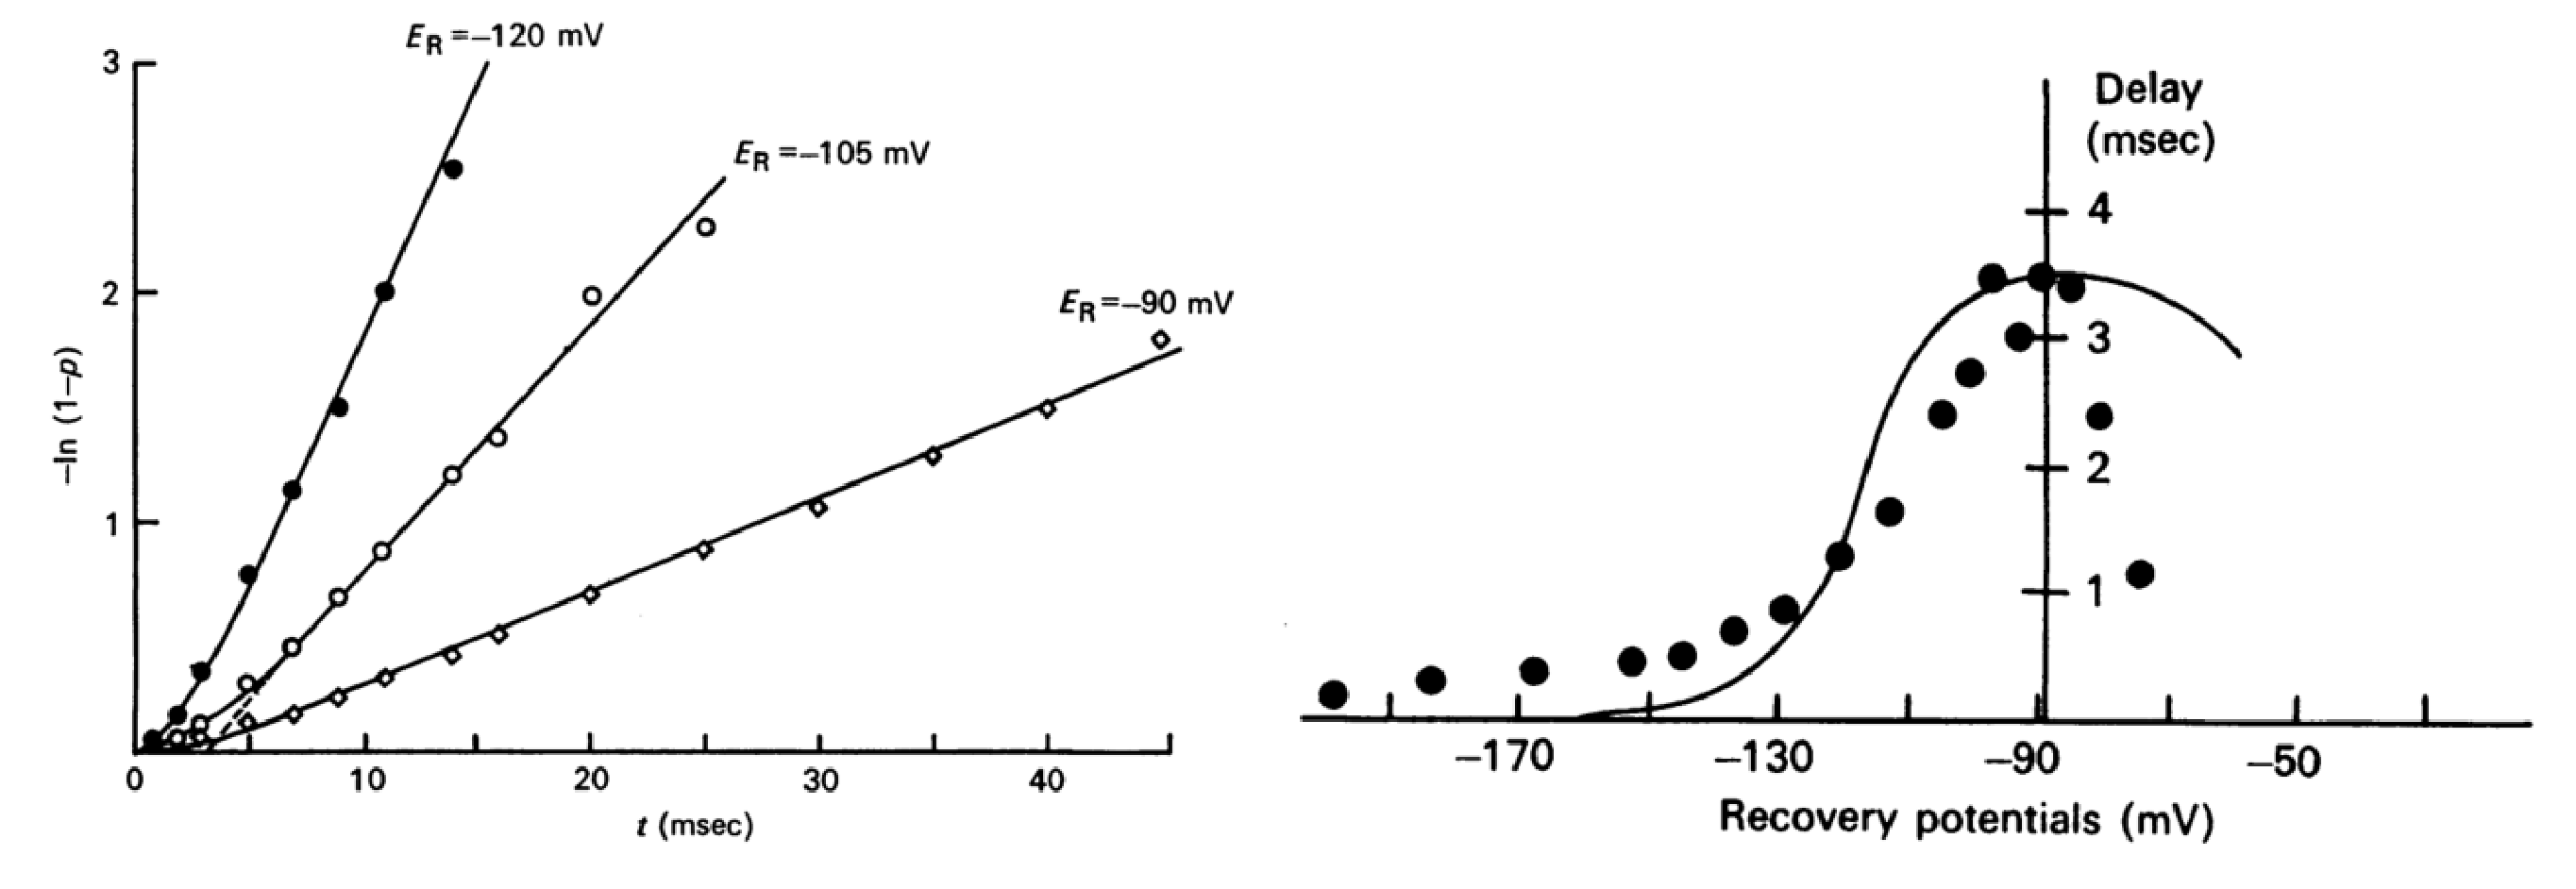
\includegraphics[height=4cm,
 angle=0]{./images/Ina_log_Chiu77.eps}} 
 \caption{Semi-logarithm plot}
\label{fig:Ina_log_Chiu77}
\end{figure}


So, Chiu suggested using the 3-state model:
\begin{equation*}
\begin{split}
&\ce{0 <=>[a_{01}][a_{10}] 1 <=>[a_{12}][a_{21}] 2}  \\
& (a_{ij} = \exp(A_{ij}V_m + B_{ij}))
\end{split}
\end{equation*}
with 0 = open; 1,2=closed state.

  The data then can be fitted using the equation of time course of recovery
  \begin{equation}\label{eqn:Po_Chiu77}
  P_0(t)/P_0(\infty) = 1 + \frac{k_2}{k_1-k_2}\exp(-k_1t) +
  \frac{k_1}{k_2-k_1}\exp(-k_2t)
  \end{equation}
  The delay can be deduced to have the following potential dependence
  \begin{equation}
  t = \frac{1}{k_2}\ln\frac{k_1}{k_1-k_2}
  \end{equation}
  The continuous lines in Fig.\ref{fig:Ina_protocol_Chiu77}(B) are fitted by
  eqn.\ref{eqn:Po_Chiu77}. 
  

\section{Begenisich-Cahalan (1980) - squid axon}
\label{sec:Ina_Begenesich1980}

\citep{begenisich1980, begenesich1980b} used rate-theory description to search
for the proper energy barriers and wells with three-barrier model, that best fit
resulting reversal potential of $\Na$ channels. About 15000 parameters sets of
well depths were tested, for each model, the current calculated from this model
were compared with I-V data, and the best result as the values shown in
Fig.\ref{fig:Ina_freenergy}(B). In the two-binding site model, the general form is given in
Fig.\ref{fig:Ina_freenergy}(A). 

\begin{figure}[hbt]

  \centerline{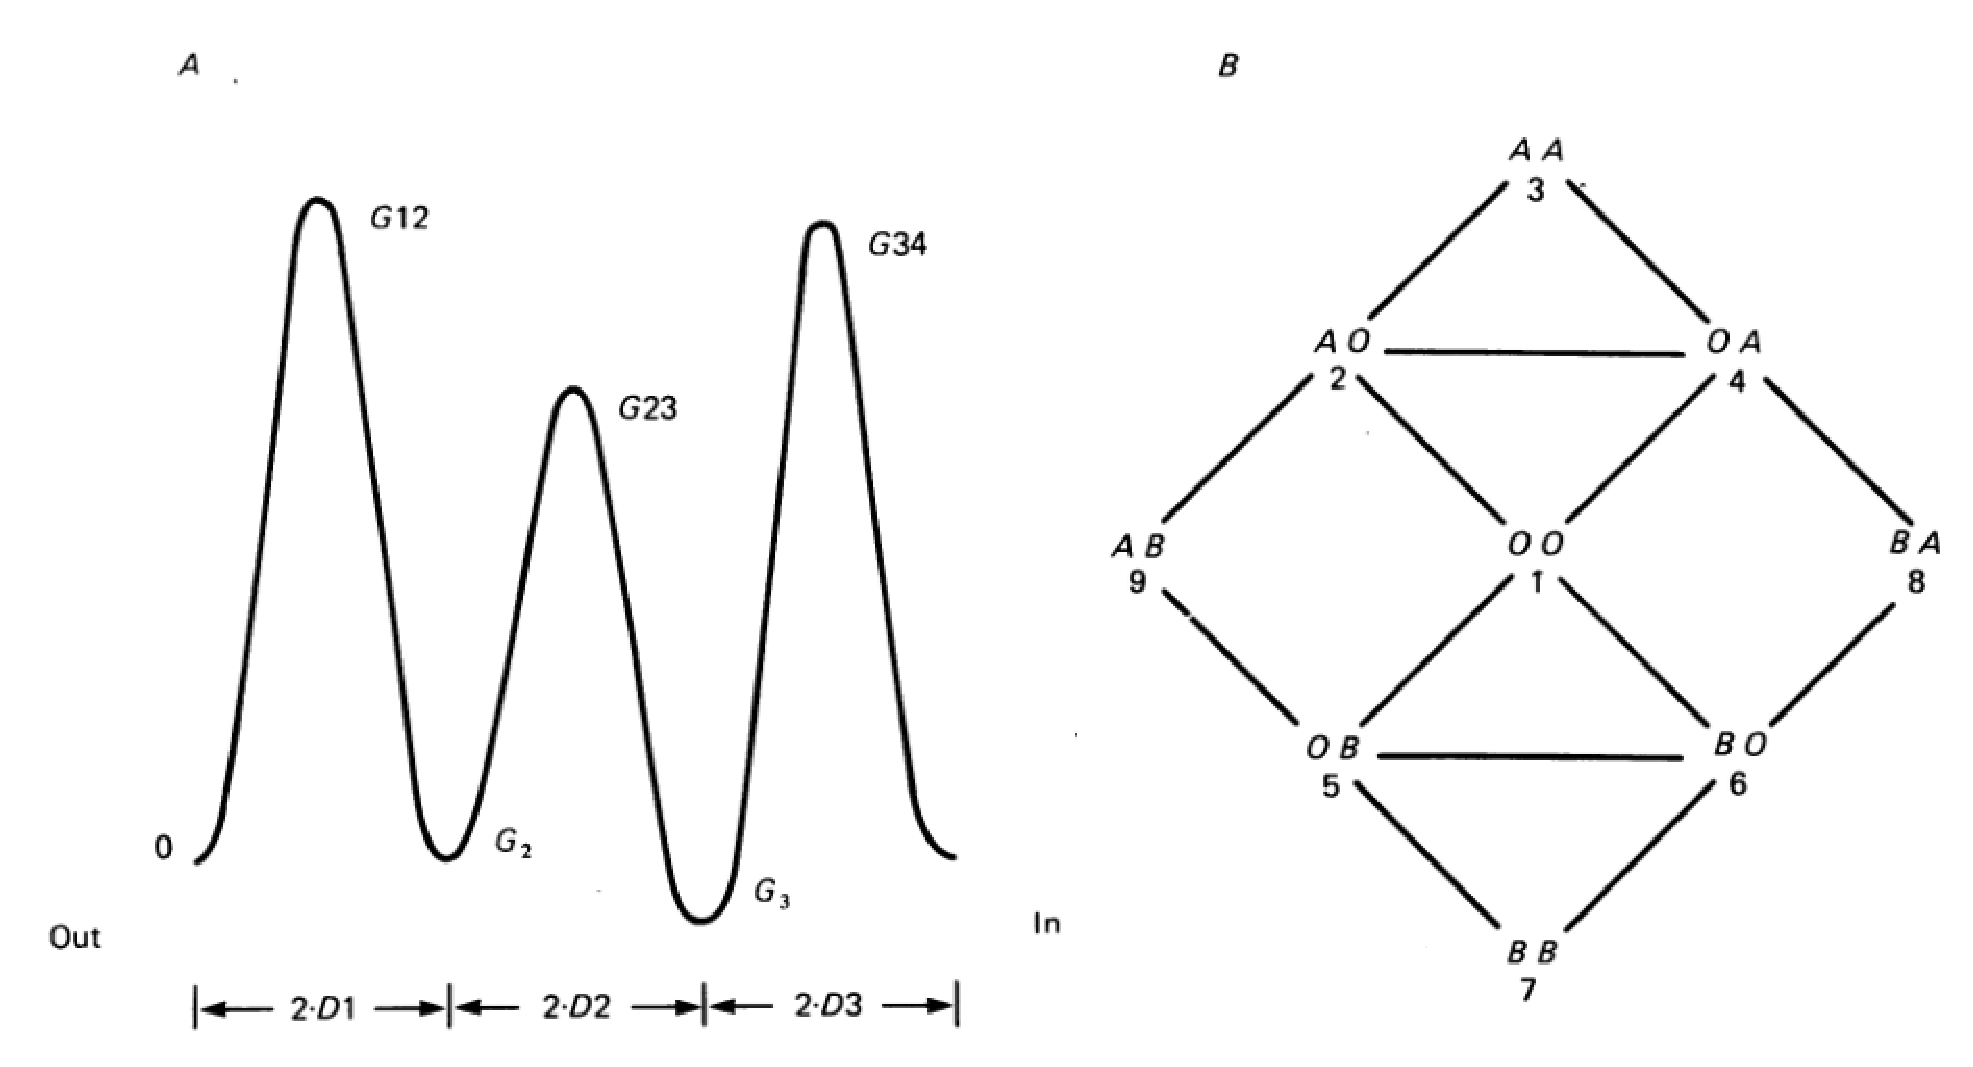
\includegraphics[height=5cm,
    angle=0]{./images/Eyring_2site-model.eps}}
  \centerline{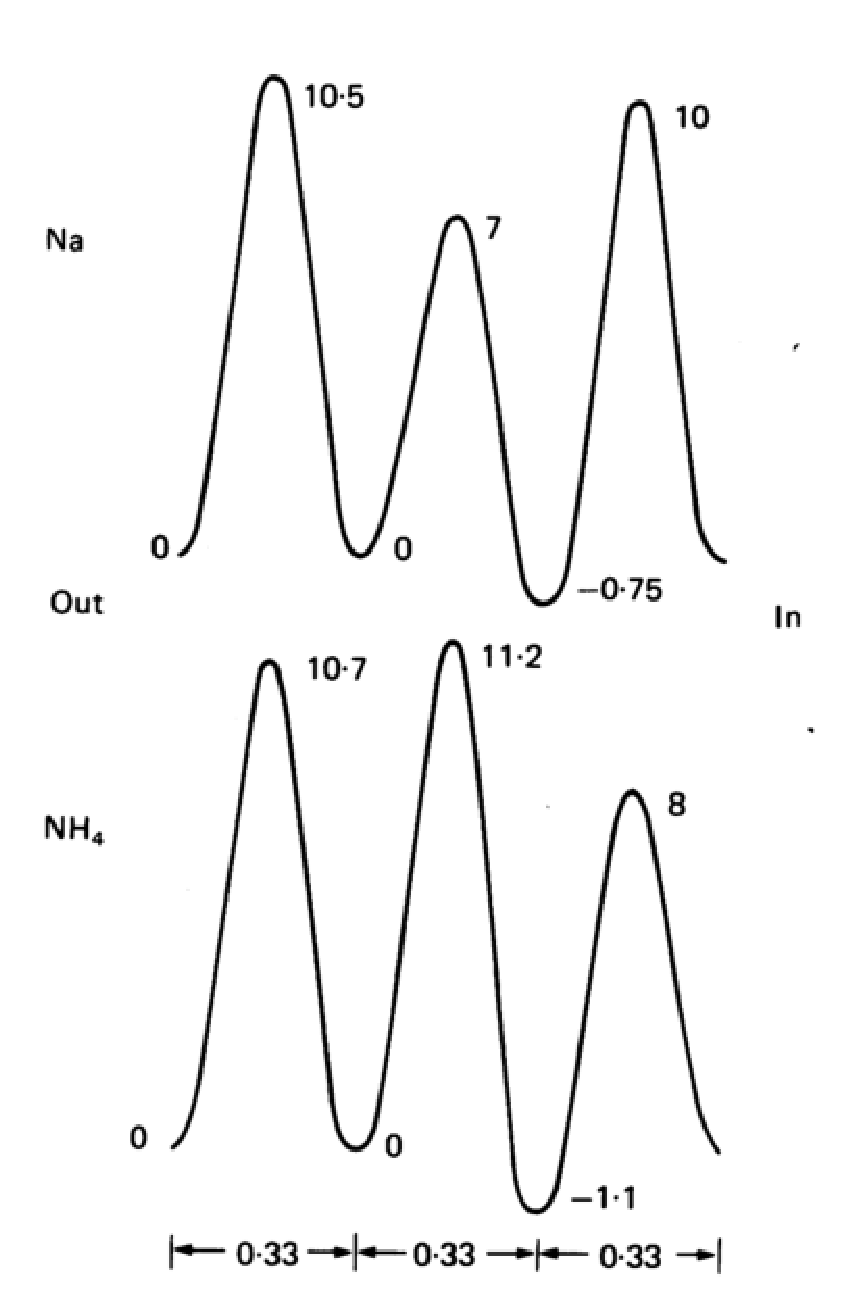
\includegraphics[height=5cm,
    angle=0]{./images/Ina_energybarrier.eps}}
\caption{(A) An arbitrary free energy profile of an ion with two-binding site
channel permeable to a single type of ion with 4 possible states. (B) If the
channel peremeate two different types of ions ($\Na$ and $\ce{NH4}$) then we
have two free energy profiles and 9 possible states}
\label{fig:Ina_freenergy}
\end{figure}

Supose there are two types of ions ($\Na$ and $\ce{NH4}$) that can permeate
through the $\Na$ channel. So, the empty state of two-binding site OO can be
filled either by ions of type A or type B or both. It's reasonable to assume
{\bf sequential binding}, i.e. ions can move to only empty site and both sites
can NOT be simultaneously occupied. This give 9 different possible states with 
9 transition-rate equations with $P_i(t)$ is the fraction of channels in state
$i$-th at time $t$
\begin{equation}
\begin{split}
\frac{dP_1(t)}{dt} &= -P_1(t) \sum^9_{j\ne 1}k_{1j} + \sum^9_{j\ne 1}
k_{j1}P_j(t) \\ 
 &\ldots \\
\frac{dP_9(t)}{dt} &= -P_9(t) \sum^9_{j\ne 9}k_{9j} + \sum^9_{j\ne 9}
k_{j9}P_j(t) \\  
\end{split}
\end{equation}

In general, there are totally 144 possible rate constants $k_{ij}$. However, in
this case, only 28 (forteen forward and forteen reverse) are non-zero. Further,
not all these rate constants are independent.

We're insterested in the steady-state solution where $dP_i/dt = 0$ and under the
conservation law: $\sum P_i = 1$. This can be written in the matrix form
$\mathbf{P}^T.\mathbf{K = 0}$, with
\begin{equation}
P = \left(\begin{array}{c} P_1 \\ P_2 \\ \ldots \\ P_9
\end{array}
 \right) \text{ and } K = \left( \begin{array}{cccc} 
 -\sum^9_{j\ne 1}k_{1j} &  k_{12} & \ldots & k_{19} \\
 \ldots \\
 k_{91} & k_{92} & \ldots & -\sum^9_{j\ne 9}k_{9j}
 \end{array}\right)
\end{equation}
$\mathbf{K}$ is the matrix where the row sum is zero. NOTE: Where necessary, the
rate constant also include the ionic concentration, or the rate constant can be
function of the ionic concentration as well.

\begin{mdframed}

Using the barrier energy (Sect.\ref{sec:eyring-rate-theory}) in the model, the
rate constants can be estimated using the {\bf principles of absolute reaction
rate theory}. E.g. the rate constant $k_{24}$ is proportional to the rate of
ionic movement from well G2 to well G3 over energy barrier G3
\begin{equation}
k_{24} = \eta \exp\left( -G_{23} + G_2 - D_2.V_m \right)
\end{equation}
The \textcolor{red}{first two terms} $G_{23}, G_2$ represent the intrinsic
(non-voltage dependent) part of the free energies (unit: $k_BT$). 

The \textcolor{red}{last term} is the contribution of the membrane potential
$V_m$, and $\eta$ is the frequency factor (unit: 1/sec). The value of $\eta$ in the usual Eyring
formulation is $k_BT/h$ (with $h$ is Planck's constant, $k_B$ is Boltzmann
constant and $T$ is temperature (Kelvin)) [NOTE: $k_BT/h \approx 5.8\times
10^{12}$ (1/s) at 10$^\circ$C]. Hill suggested that this factor $\eta$ should be
replaced by $D/(RA)$ with $D$ is inoic diffusion constant, $R$ is capture
distance (pore), and $A$ is deBroglie wave-length of reacting species. Then, for
$\Na$ ions (D=$1.5\times10^{-5}$ cm$^2$/s, R=2.4$\AA$), the value should be $3\times
10^{11}$ (1/s). However, an exact value for $\eta $ is not important to be able
to use this approach.
\end{mdframed}

After having the rate constants and steady-state probabilities $P_i(\infty)$,
the steady-state flux of each type of ion (A and B) can be calculated. Here, the
middle barrier is chosen
\begin{equation}
\begin{split}
F_A = P_4 k_{42} - P_2 k_{24} \\
F_B = P_5 k_{56} - P_6 k_{65} \\
\end{split}
\end{equation}

The permeability $P_\text{NH4}/P_\na$ was calculated using GHK equation
\begin{equation}
\begin{split}
P_\text{NH4}/P_\na	 = \frac{[\Na]_o}{[NH4]_i} \exp(\frac{-E_\rev.F}{RT}) \\
P_\text{NH4}/P_\na	 = \frac{[\Na]_i}{[NH4]_o} \exp(\frac{E_\rev.F}{RT}) \\
\end{split}
\end{equation}


\section{Armstrong (1981)}
\label{sec:Ina_Armstrong1981}

\subsection{activation}

\citep{armstrong1981}  found that the sigmoidal activation curve implies the
existence of at least 3 closed states. They suggested sequential multi-state
binding, started with 5 closed state (the number is necessary to fit the
activation as a sigmoidal and also achieve the appropriate time course) and one
open state and use only one gating variable
\begin{equation}
\ce{X6 <->[a_5][\beta_5] X5 <->[a_4][\beta_4] X4 <->[a_3][\beta_3] X3
<->[a_2][\beta_2] X2 <->[a_1][\beta_1] \text{O}}
\end{equation}
The choice of 5 rather than 4 or 6 states, as it gives better fit to the data.
Nevertheless, the model is still empirical. 

The rate constants in the first four steps are
fast (X6$\rightarrow$X2), and the last one (X2$\rightarrow$O) is slow (to
generate fast and intermediate components).

\subsection{inactivation}

Model for inactivation, after a time, inactivate occur by the reaction
X$_1^{*}\rightarrow$ X$_1$Z. The state X$_1$Z is fuly open (which is the
conducting state), and entry to this state only occur after the channel opens.
Under membrane repolarization, the channels quickly switch to X$_2$Z (partially
close). In this model, the maximum open fraction is approximately 0.7 (as
mostly channels open and conduct at least momentarily before thay inactivate,
and a small fraction follow the path X$_2\rightarrow$X$_2$Z).


\section{Horn-Vandenberg (1984) - tissue-culture GH3 cell}
\label{sec:Ina_Horn1984}

\citep{Horn1984} created a model based on tissue-cultured GH3 cell (a clonal
line from rat pituitary gland - Sect.\ref{sec:pituitary-gland}). 
By testing current via a single channel only, it seems that there is only one 
opening state, as the dwell-time history shows only one peak. 
They suggested that Hodgkin-Huxley model and any model requiring a channel
to open before inactivating is unacceptable.


They also want to know which classes of models are not consistent with
experimental data.
Fig.\ref{fig:Ina_Vandenberg} showed different inactivation time constant at
different test pulses: $\tau_h$ = 8.1, 3.1 and 1.9 (ms) for -20mV, 0mV and
+20mV. \citep{Vandenberg1984} showed the whole-cell rate of inactivation is
voltage-dependence with $\tau_h$ varied e-fold per 26 mV.


\begin{figure}[hbt]
 \centerline{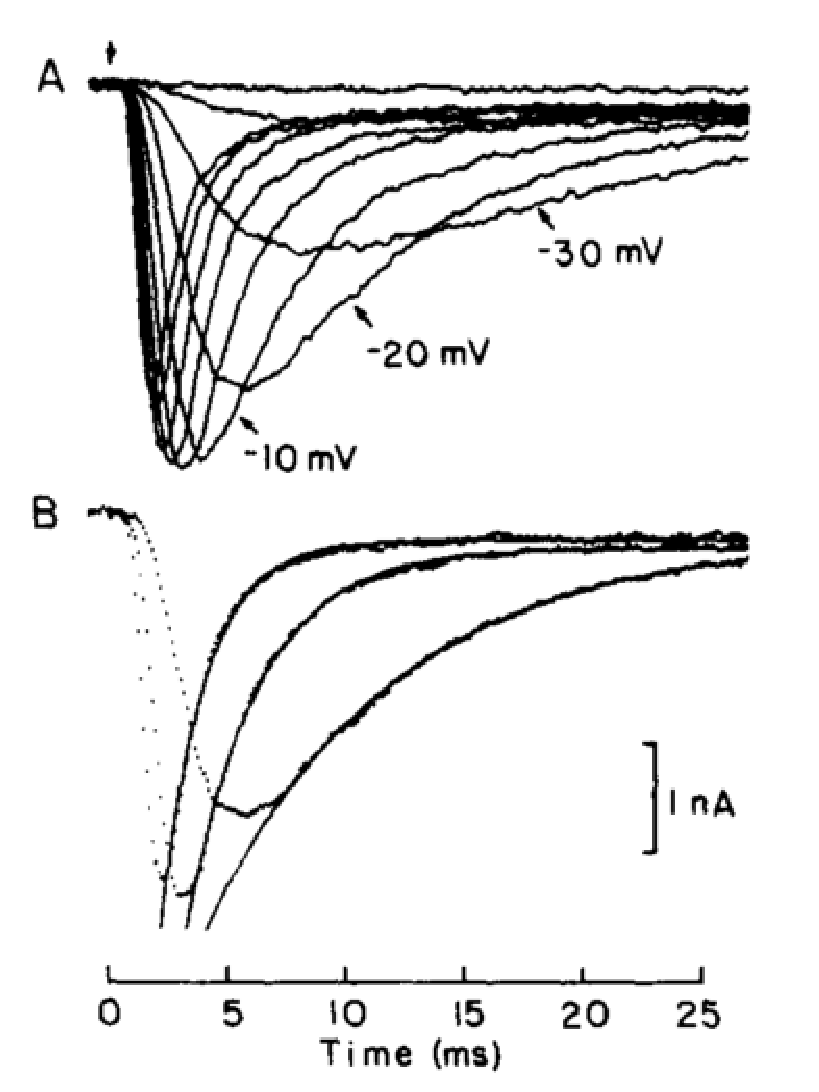
\includegraphics[height=6cm,
 angle=0]{./images/Ina_Vandenberg1984.eps}}
\caption{Macroscopic sodium currents (A) elicited in response to +29ms voltage
step from -50mV to +40 mV with 10-mV increment from holding potential -80mV;
(B) currents for test pulse -20, 0, and +20 mV; together with a single
exponential fit to the falling phase \citep{Vandenberg1984}}
\label{fig:Ina_Vandenberg}
\end{figure}


The number of arrangement of closed states of the $\Na$ channel are not known.
They tested 25 different configuration for 5-state Markov model. The basic one
is given in Fig.\ref{fig:Ina_scheme1_Horn1984}. The inactivated state is
different from other closed states in 2 ways: (1) the channels at holding
potentials stay in one of the closed states; (2) the rate for leaving I-state
are small at activating voltages (and end up in the I-state after the
depolarization). 

As there is no certain about the initial probability distribution among the
states at rest, the assumption was: at time zero, 98\% of the channels are in C1
and 2\% are in C2. With 10 rate constants, only 9 are need to be estimated as
the last one can be calculated from microscopic reversibility.

\begin{figure}[hbt]
 \centerline{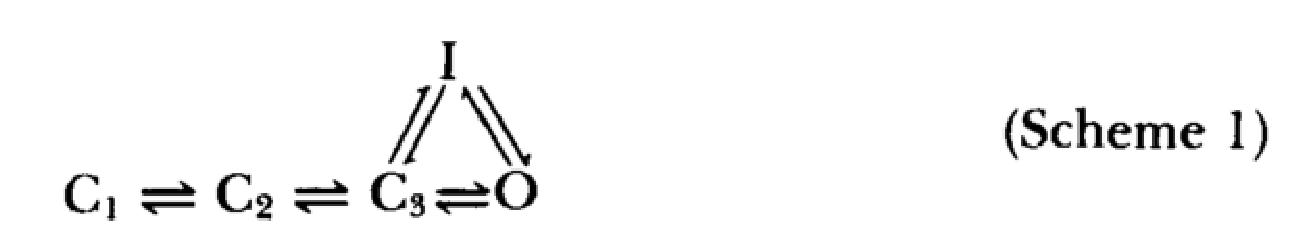
\includegraphics[height=2cm,
 angle=0]{./images/Na_scheme1_Horn1984.eps}}
\caption{A simple Markov-based model for $\Na$ channel}
\label{fig:Ina_scheme1_Horn1984}
\end{figure}



\section{Rose-Hindmarsh (1989)}
\label{sec:Ina_Rose-Hindmarsh-1989}

\begin{equation}
I_\na = \bar{g_\na} \times m_\infty^3(\Vm) \times (0.85 - n) \times (\Vm -
E_\na)
\end{equation}

Sodium activation is assumed instantaneous, i.e. using $m_\infty$, and the
kinetics is similar to original HH-model (Sect.\ref{sec:Ina_Hodgkin-Huxley},
except it shifts $\Vm$-dependent to $\sigma_i$ (i=m, n).
  
\section{Hindmarsh - Rush (1989)}
\label{sec:Ina_Hindmarsh-Rush-1989}

Hindmarsh-Rush developed the model for $\Na$ current in
thalamic neuron (Sect.\ref{sec:Hindmarsh-Rush_model}) using the Hodgkin-Huxley formula
for gating kinetics, with a shift in Voltage-dependency upward along the axis.


\section{Wang et al. (1991) - thalamic neuron}
\label{sec:Ina_Wang1991}

\section{Rush-Rinzel (1994) - thalamic neuron}
\label{sec:Ina_Rush-Rinzel1994}

The transient Na current model in Rush and Rinzel (1994 -
Sect.\ref{sec:Rush-Rinzel-1994}) is based on that developed by Hindmarsh-Rush
(1989) - Sect.\ref{sec:Ina_Hindmarsh-Rush-1989}).

They simplified further and replace 
\begin{itemize}
  
  \item replace sodium inactivation gating variable $h$ by a linear function of
  potassium activation $n$ gating, i.e. $h = 0.85 - n$, i.e. to emulate the
  effect of potassium A-current shift the threshold for sodium spike.
%TODO: modeling effect of K+ on Na+ gating

So, sodium inactivation is not explicitly included.
To match recent experimental findings that $\tau_h$ is approximately constant at
30 ms for V $>$ -40 mV (Huguenard and McCormick 1992).

  
  \item sodium activation is assumed instantaneous, i.e. using $m_\infty$, and 
  the kinetics is similar to original HH-model
  (Sect.\ref{sec:Ina_Hodgkin-Huxley}, except it shifts $\Vm$-dependent to
  $\sigma_i$ (i=m, n), as in Sect.\ref{sec:Ina_Rose-Hindmarsh-1989}
  
\end{itemize}

\begin{equation}
I_\na = \bar{g_\na} \times m_\infty^3(\Vm) \times (0.85 - n) \times (\Vm -
E_\na)
\end{equation}


\section{Martina-Jonas (1997): Nat in interneurons vs. principal neurons}
\label{sec:Nat-Martina-Jonas-1997-interneuron-DG-basket-cells}
\label{sec:Nat-Martina-Jonas-1997-pyramidal-CA1}

Martina, Jonas (1997) studied the functional difference of $\Na$ channels
between interneurons, e.g. dentate gyrus basket cell
(Sect.\ref{sec:dentate_gyrus}, Sect.\ref{sec:basket-cell}); and principal
neurons, e.g. CA1 pyramial neuron of rat hippocampal slices.

Recording were done on a membrane nucleated patch of surface area about 78.5
$\mum^2$. Test pulses: from -80mV to +40mV; solution: 84mM $[\Na]_i$

\begin{table}[hbt]
\begin{center}
    \begin{tabular}{lcc}
        \hline
        & DG basket cells &  CA1 pyramidal neurons \\
        \hline \hline
        peak current & at about -20mV & the same \\
        Erev (membrane patch) & +15.6mV & +15mV \\
        Erev (linear interpolation to physiological value) & \\
        using 12 $[\Na]_i$ & +63.3 mV & +60.6 mV  \\
         and 4mM  & +70.0 mV & +75.1 mV \\
        \hline
        activation & k=11.5 (mV) & k=11.8 (mV) \\
        & Vh = -25.1 (mV) & Vh = -23.9 (mV) \\
        \hline
        time constant activation (-30mV to +40mV) &  the same & the same \\
        \hline
        deactivation time constant  & faster in BC & \\
        (tail current decay) &  0.12ms at -40mV & 0.20 ms at -40mV \\
        \hline
        inactivation & k=6.7 & k=10.7 \\
        & Vh = -58.2 (mV) & Vh = -62.9 (mV) \\
        \hline
    \end{tabular}
\end{center}
\caption{Comparison of Nat current in interneurons (e.g. DG basket cells) vs.
principal neuron (e.g. CA1 pyramidal neurons)}
\label{tab:Nat-interneuron-vs-pyramidal-neuron}
\end{table}

\begin{enumerate}
  \item Nat interneurons: 
\end{enumerate}


\section{Colbert - Pan (2002)}
\label{sec:NaT-Colbert-2002}

The  model is developed for Sect.\ref{sec:Colbert-Pan-2002}.

\begin{equation}
g_\na = \bar{g_\na} m^3 h
\end{equation}

Parameters were determined using least-square fit to axonal $\Na$ current
ensemble average. $\bar{g_\na} = 0.0336$ S/cm$^2$. 

However, the model was chosen so that only 35\% open maximum, i.e. max($m^3h$) =
0.35, thus the peak $\Na$ conductance is about 12 mS/cm$^2$.


Room Temperature: 23$\pm$ 0.5$^\circ$C.

To construct activation curves, we held patches at -100 mV and stepped
them to -70, -60, -50, -45, -40, -30, -20, -10 and 0 mV. 

The peak current at each potential was then converted to a chord conductance
assuming a Na+ reversal potential of +55 mV.

Least-square fit was made using single Boltzmann function: yield a half
activation $V_{1/2}$ and slope $k$.


Somatic patches included K+ channel blockers to block the fast transient K+
currents. They included axonal and initial segment patches without
blockers in the analysis because they lacked the fast transient current, and the
relatively small sustained current reached a maximum well after the peak of the
Na+ current, except for few cases (n=2 for axon, n=3 for initial segment).

For inactivation curves, we held patches at potentials between -100 and -30 mV
for 3 s and then stepped them to 0 mV to evoke currents.
We normalized
data to the maximum current (from -100 mV) and fit them to a negative
Boltzmann curve.






\section{Wolf et al. (2005) - NaT (CA1 hippocampal pyramidal neuron)}
\label{sec:NaT-Wolf-2005}

\citep{wolf2005} (Sect.\ref{sec:Wolf-2005-MSN}) used data to fit NaT from rat
hippocampal CA1 pyramidal neurons provided by Martina-Jonas (1997) -
Sect.\ref{sec:Martina-Jonas-1997}. \textcolor{red}{Using voltage-clamp, Fig.1 in
the paper, with holding potential -90mV; and 50ms test-pulse from -80mV to
+40mV: the peak is at -20mV (using [$\Na$]i = 84 mM)}
 
\begin{equation}
I  = \bar{g} m^x h^y (V_m - E_\rev)
\end{equation}

Two diffent kinetics are used:
\begin{itemize}
  \item If $V_m \le -40$(mV)
  
\begin{equation}
\tau_m = 0.025 + 0.14 \times \exp[(v + 40)/10]
\end{equation}
  
  \item If $V_m \ge -40$(mV)

\begin{equation}
\tau_m = 0.02 + 0.145 \times \exp[-(V+40)/10]
\end{equation}
\end{itemize}

\section{Wolf et al. (2005) - NaP (entorhinal cortical stellate cells)}
\label{sec:NaP-Wolf-2005}

\citep{wolf2005} (Sect.\ref{sec:Wolf-2005-MSN}) used data to fit NaP 
\begin{enumerate}
  \item inactivation: from steady-state I-V curve from entorhinal cortical
  stellate cells (Magistretti- Alonso, 1999) - Sect.\ref{sec:Magistretti-Alonso-1999}
  
  \item activation: a computational model of a rat layer 2/3 pyramidal neuron
  (Traub et al., 2003)
\end{enumerate}


\chapter{Na model (cardiac)}

Until early 1980s, direct measurements of the excitatory sodium current (Ina) in
heart had been difficult because the complex multicellular organization of
cardiac muscle limits the degree of spatial and temporal uniformity that can be
achieved with the voltage clamp technique.

\begin{enumerate}
  \item Longitudinal non-uniformities arise because a point source of
current must be used. 

Voltage non-uniformities can be tolerated for relatively small membrane
currents (Kass, Siegelbaum \& Tsien, 1979) but become severe when membrane
current flow is intense, as during the excitatory sodium current.

Voltage non-uniformity was minimized by partially removing the external sodium
to reduce the size of the current, and by lowering the temperature to slow the
current kinetics. Under these conditions, the recorded currents satisfy a number
of criteria for adequate voltage control.

  \item Radial non-uniformities are introduced in many preparations by the
  presence of narrow intercellular spaces which places a significant external
  resistance in series with much of the total membrane.
  
\end{enumerate}

Low temperatures were necessary to improve temporal resolution of INa.
Typically, it starts at room temperature (about 24$^\circ$C) and bath
temperature gradually lowered to the desired final level.
Once a stable condition was obtained, the superfusate was exchanged for one
containing low sodium (to reduce INa current). 


\section{Purkinje fibers}

NOTE: Purkinje fibres from rabbit ventricle have fewer morphological
complexities than other naturally occurring cardiac preparations.
They lack transverse tubules, unlike mammalian ventricular muscle, and have
fairly wide (1 $\mum$) intercellular clefts, unlike sheep Purkinje fibres and
frog myocardium. Cable analysis showed the rabbit Purkinje fibre to behave as a
simple RC cable with an extremely low external series resistance.

Radial non-uniformities in membrane potential and potassium
ion concentration during voltage clamp polarizations were considerably smaller
in Purkinje fiber of rabbit ventricle than those found in ungulate Purkinje
fibres in similar experiments.

Earlier studies (until 1970s) of INa in the rabbit Purkinje fibre using the
{\bf double sucrose gap} were complicated by poor viability of the preparations
and by the presence of large extracellular shunt currents.



\section{Hodgkin-Huxley-type formula}
\label{sec:Hodgkin-Huxley-Na-models-cardiac}


\subsection{Dudel, Rudel (1969) - Purkinje fiber (cardiac)}
\label{sec:Ina_Dudel-Rudel-1969-Purkinje-fiber}

Using the same assumptions and approximation by Hodgkin and Huxley,
eq.\ref{eq:HH-Na-conductance-reduced-form},  the rate constants are estimated -
Sect.\ref{sec:rate-function-simple-exponential-form}

UNIT of rate constants (in ms) 
\begin{equation}
\begin{split}
\alpha_m &= \frac{0.55}{\exp(\frac{\Vm - (55)}{10}) + 1} \\
\beta_m &= \frac{0.015 \left( \Vm - (-16) \right)}{\exp(\frac{\Vm - (-6)}{2})
- 1} \\
\beta_h &= \frac{0.108}{\exp\left(- \frac{\Vm - (-50)}{15}\right) + 1 } \\
& \text{ $\alpha_h$ and $h_\infty$ are zero when $\Vm > -100$ mV}
\end{split}
\end{equation}

\textcolor{red}{NOTE}: the absolute of the rate constants measured by Dudel
and Rudel for the cooled (low temperature) Purkjie fiber are
\begin{enumerate}
  \item lower than that in Hodgkin-Huxley
  model for squid giant axon about 10x
  \item lower than that in Frankenhaenser data for myelinated nerve fiber about
  100x (i.e. two orders of magnitude)
\end{enumerate}
There can be imperfection in the voltage-clamp protocols in the study, making
the rise is slower. 

\subsection{Colatsky (1980)}
\label{sec:Ina_Colatsky-1980}

Colatsky (1980) also use permeability formula, similar to that in Frankenhaenser
(1960) (Sect.\ref{sec:Ina_Frankenhaeuser-1960}) to model INa. 
\begin{equation}
P_\na= \frac{I_\na. R.T}{F^2 . \Vm . [\Na]_o}
\frac{\exp(\Vm.F/(RT)) - 1}{\exp((\Vm-E_\na).F/(RT)) - 1}
\end{equation}


Low temperature was used to improve the temporal resolution of INa, i.e.
kinetics slower. The total recorded current is the result of 3 components; in
that each can be subtracted out from the trace. Also, the late inward Ca2+
current can be reduced by using magnesium ($\Mg$) in the bath solution.
In such condition, the ionic current recorded on depolarization consisted of INa
and a small amount of leak.

PROTOCOLS: It uses two-micro-electrode voltage clamp technique of Deck, Kern \&
Trautwein (1964) with minor modifications (Tsien, 1974).
Lower sodium level is used, e.g. 10-13\% less than normal. 

NOTE: the I-V curves incorporate differences in both driving force and resting
inactivation
\begin{itemize}
  \item at 20mM $[\Na]_o$, and holding potential -82 mV: 
  
  
  the Erev is +2.5 mV, which get the peak INa at -26$\pm$2 mV
  
  \item at 155 mM $[\Na]_o$, and holding potential -71 mV: the Erev is +44 mV,
  which get the peak INa at -15$\pm$1 mV.
  
\end{itemize}

The measured permeability $P_\na$ is then normalized to the maximum permeability
calculated from each run.
\begin{itemize}
  \item $P_\na$ also show sigmoidal relationship with step potential;
  with almost no activation at -55 mV; to nearly full activation at -10 mV.  
\end{itemize}


\subsection{Ebihara-Johnson (1980) - TTX-sensitive, fast INa on
tissue-cultured Purkinje fiber of embryonic chicken heart (37$^\circ$C)}
\label{sec:Ina_E-J-model}

In Purkinje fiber, the time course of inactivation was found to be fast, with
time constant for inactivation of sodium current was estimated less than 1-2 ms.
However, the developed voltage clamp did provide sufficient voltage control at
the first 10ms after depolarization step (Deck, Kern and Trautwein (1964)
method), i.e. voltage step did not complete less than a milisecond. 

Early data in sheep Purkinje fiber at 8$^\circ$C showed the voltage and
time-dependence rate coefficients of activation and inactivation is similar in
form to that found in squid giant axon (Sect.\ref{sec:Ina_Hodgkin-Huxley}) at
15$^\circ$; but \textcolor{blue}{the one in Purkinje fiber is about an order of
magnitude slower}.
\begin{enumerate}
  
  \item Temperature dependence of resting membrane potential in Purkinje fiber:
  \begin{itemize}
    \item at about 20$^\circ$C: Vrest decrease a little
    \item at 10-20$^\circ$C: the fiber increasingly depolarize
    \item at < 10$^\circ$C: Vrest is about -30mV to -10mV below.
  \end{itemize}
    
  \item   
\end{enumerate}

A previous study was Dudel, Rudel (1969) -
Sect.\ref{sec:Ina_Dudel-Rudel-1969-Purkinje-fiber} - cooled very small Purkinje
fiber down to 4-5$^\circ$C, to separate fast sodium current from capacitive
current. REVIEW:
\begin{itemize}
  \item    NOTE: This also affect resting membrane potential, i.e. Vrest decreased -30mV
  at this low temperature. 
  
  \item   They found that $h$ inactivation gate has a remarkable potential depdenence
  with $h=1$ at Vm = +180 mV; and $h=0$ at -100mV. 
 
  
  The time course of the removal of inactivation showed a similar dependence on
  conditioning prepotential and time to that found for the squid giant axon.
  
  The decay of the sodium current flowing after depolarization can be fitted by
  two time constants rather than one.
  
\end{itemize}
 
\citep{ebihara1980fsc}

\citep{ebihara1980iic} studied kinetics of transient INa current in a tissue of
11-day embryonic heart cells at 37$^\circ$C. They showed that the kinetics is
similar to that found in nerve.
\begin{itemize}
  \item time constant of inactivation $\tau_h$ seems independent of voltage for
  large preparation; and then steeply voltage dependent with less spatial
  non-uniformity within the preparation, i.e. $\tau_h = 2.14$(ms) at -40mV; and
  0.18 (ms) at -5 mV.
  
  \item 
\end{itemize}
  
In this study, it suggested that at 37$^\circ$C the sodium carrying system
should be almost entirely inactivated ($h=0$) when the action potential reaches
its   Vrest. It was showed that using two-electrode give better measurement of
the Na current. Using two-microelectrode, the data from 11-day-old embryonic
heart cells at 37$^\circ$C of chicken was measured.
\begin{enumerate}
  \item Sect.\ref{sec:voltage-clamp-protocol-estimate-inactivation-single-pulse}
  to estimate $h_\infty$
  
  $h=1$ when $\Vm < -90$ (mV), i.e. current saturated or all channel is open
  when depolarized from -90mV to -20mV.
  
  $h=0$ when $\Vm > -50$ (mV), i.e. no current is observed if conditioning
  prepulse at $\Vm > -50$ (mV) for 300ms. 
  
  In overall, the shape of $h_\infty$ is fitted with Boltzmann curve with $V_h
  = -69$ (mV) and $k=6.3$ (mV).
  
  \item time constant of inactivation $\tau_h$ was found in Fig. 6
  
  \item time course of activation was too fast to be separated from capacitive
  current when step potential > -10 mV. 
\end{enumerate}

\citep{ebihara1980fsc} formulated the fast $\Na$ current by the equation using
Hodgkin-Huxley original formula (NOTE: E-J model)
\begin{equation}
I_\na = \bar{g_\na} m^3 h (V_m - E_\na)
\end{equation}
with $E_\na = 29$ (mV) as the $[\Na]_i = 40$ (mM) in chicken
embryo heart cells. $\bar{g_\na} = 23$ (mS/cm$^2$).
\textcolor{red}{The peak sodium conductance, using voltage clamp with
holding-potential at -60mV, is shown in Fig.2 of the paper (peak about -10mV)}.

Compared to squid at 15$^\circ$C: the functions of potentials are similar,
except the magnitudes are larger (faster).

NOTE: There is a type for $\alpha_m$ in the paper
\begin{equation}
\begin{split}
\alpha_m &= \frac{0.32 (V_m - (-47.13))}{1 - \exp \left( (V_m - (-47.13))/(-1.0)
\right)}
\\
\beta_m &= 0.08 \times \exp \left( V_m / (-11) \right) 
\end{split}
\end{equation}

If $V_m > -40$ (mV) then
\begin{equation}
\begin{split}
\alpha_h &= 0 \\
\beta_h &= \frac{1}{0.13 \exp \left( (V_m - (-10.66))/(-11.1) \right)}
\end{split}
\end{equation}

If $V_m < -40$ (mV) then
\begin{equation}
\begin{split}
\alpha_h = 0.135 \exp \left( -(V_m - (-80))/ 6.8 \right) \\
\beta_h = 3.56 \exp \left( 0.079 V_m \right) + 3.1 \times 10^5 \exp \left( 0.35
V_m \right)
\end{split}
\end{equation}

NOTE: \citep{spach1995} used $E_\na = 33.45$ (mV), and $\bar{g_\na} =
28$mS/cm$^2$.
\section{Haas et al. (1970) - atrial (4-7$^\circ$C)}
\label{sec:Ina_Haas}

The kinetics of Na current was studied at 4-7$^\circ$C, in atrial
\citep{haas1971}. At this temperature, the time-constant for
recovery from inactivation is slow, i.e. from 100ms to 600ms. 

\textcolor{red}{The peak conductance using voltage-clamp with holding potential
-60mV; occurs at -40mV, Fig.4 in the original paper.}

Haas et al. suggested the inactivation curve has two different time constants,
and thus should be fitted with two inactivation variables, represented by the
$h$ as the fraction of open inactivated-gate-type-1; and $j$ as the fraction of
open inactivated-gate-type-2.

\begin{equation}
g_\na  = \bar{g_\na}.m^3.h.j
\end{equation}
\section{Beeler-Reuter (1977) - heart}
\label{sec:Ina_Beeler-Reuter_1977}

\textcolor{red}{Temperature is important in parameter difference. There are two
temperatures being used: room temperature (25$^\circ$C or 295K) and body
temperature (37$^\circ$C or 310 K)}. However, applying voltage-clamp technique
to cardiac myocyte at normal temperatures was currently limited. So, the
activation parameter, $m$ was adopted from squid axon by Hodgkin-Huxley model
\citep{hodgkin1952ap}.

The inactivation process is expected to be completed within 10msec, while the
re-activation from the inactivation occurs at a much slower time-scale. As the
re-activation process is thus assumed to occur via 2 time-course, the fast one
($h$) and the slower one ($j$). The inclusion of $j$ was based on
\citep{haas1971} (Sect.\ref{sec:Ina_Haas}). The value for $\tau_j$ was chosen by
matching the data of \citep{gettes1974} (data from
\textcolor{red}{right-ventricular papillary muscle of guinea-pig, measured at
37$^\circ$C, } using double-pulse protocol with a conditioning action potential)
for the potential $< -60$ mV, Fig.\ref{fig:Na_tau_j_Gettes1974}, and then bend
the curve to the right side (more positive potential) to be roughly parallel to
$\tau_h$.

\begin{figure}[hbt]
 \centerline{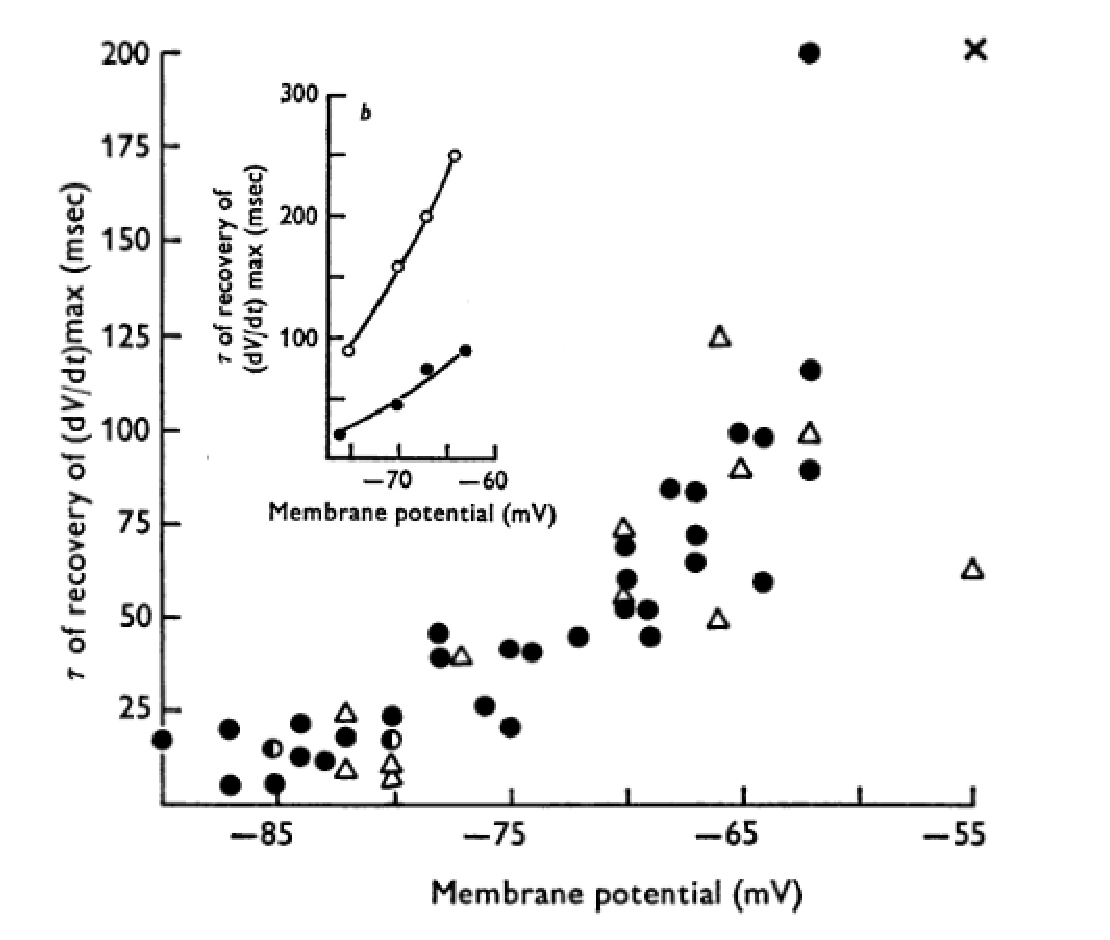
\includegraphics[height=7cm,
 angle=0]{./images/Na_tau_j_Gettes1974.eps}} 
 \caption{Time course of recovery of (dV/dt)max after a conditioning AP: filled
 circle \protect\pie{360} = guinea-pig papillary muscle, half-filled circle
 \protect\pie{-180} = sheep ventricular trabecula, crosses (x) = pig ventricular
 trabecula, open triangles $\triangle$ = Purkinje fiber from one calf and three
 sheep}
\label{fig:Na_tau_j_Gettes1974}
\end{figure}


It has been showed that the basic kinetic characteristics of $I_\na$ are similar
in ventricular cells across species \citep{hanck1995}. In cardiac cells,
Beeler-Reuter formula is based on \citep{haas1971}:
\begin{equation}
I_\na = g_\na m^3 h j (V_m-E_\na)
\end{equation}
with
\begin{enumerate}
  \item Beeler-Reuter (1977): $g_\na= 4$ (mS/cm$^2$), $E_\na = 50$ (mV),
  Fig.\ref{fig:beeler_reuter_3}.
  
  \item LR-1 (1991 - derived from cardiac cell of chicken embryo): $g_\na=23$
  (mS/cm$^2$), $E_\na=54.4$ (mV) (based on $[\Na]_i=18$ mM) to keep the peak
  $\bar{i_\na}=400 (\muA/\muF)$ 
  \begin{eqnarray}
  \alpha_m = \frac{a_1 (V_m - V_{half,1} )}{1-\exp((V_m - V_{half,1})/b_2)} \\
  \beta_m = a_3 \exp((V_m-V_{half,2})/b_3) \\
  \end{eqnarray}
  with $a_1=0.32, V_{half,1}=-47.13, V_{half,2} = 0, b_2=-10, b_3=-11$.
  
  If $V_m \ge -40$ (mV)
  \begin{eqnarray}
  \alpha_h = 0 ;   \beta_h = \frac{1}{0.13(1+\exp((V_m - V_{half,3})/(-11.1)))}
  \\
  \alpha_j = 0 ;   \beta_j = \frac{0.3\exp(-2.535\e{-7} V_m)}{1+\exp(-0.1(V_m -
  (-32)))}
  \end{eqnarray}
  with $V_{half,3}=-10.66$.
  
  If $V_m < -40$ (mV)
  \begin{eqnarray*}
  \alpha_h = && 0.135 \exp((V_m-(-80))/(-6.8)) \\
  \beta_h = &&3.56 \exp(0.079 V_m) + 3.1\e{5} \exp(0.35 V_m) \\
  \alpha_j = &&\frac{V_m+37.78}{1+\exp(0.311(V_m+79.23))} \\
       &&\left(-1.2714\e{5} \exp(0.2444V_m) - 3.474\e{-5} \exp(-0.04391 V_m)
       \right)
  \\
  \beta_j = &&\frac{0.1212 \exp(-0.01052 V_m)}{1+ \exp(-0.1378(V_m+40.14))}
  \end{eqnarray*}
  NOTE: The reason to use two different formulas is that $h_\infty$ is found to
  be zero when $V_m \ge -50 $mV. The dynamic of $j$ is obtained by setting
  $j_\infty = h_\infty$.
  
  \item LR-2 (1994 - guinea pig ventricular myocyte, 37$^\circ$C): $g_\na=16$
  (mS/cm$^2$), $E_\na=70$ (mV) to keep the peak $\bar{i_\na}=380 (\muA/\muF)$
  
  \item Pandit {\it et al.} \citep{pandit2001} (rat, 25$^\circ$C): 
  (Sect.\ref{sec:pandit_2001_rat}): $g_\na = 0.8\muS = 8$mS/$\muF$ = 8
  mS/cm$^2$ (as capacitance C$_m$ = 10$^{-4} \muF$).
  
  \begin{eqnarray*}
  m_\infty = \frac{1}{1+ e^{(V+45)/-6.5}} \\
  h_\infty = j_\infty = \frac{1}{1 + e^{(V+76.1)/6.07}} \\
  \frac{dm}{dt} = \frac{m_\infty - m}{\tau_m} \\
  \frac{dh}{dt} = \frac{h_\infty - h}{\tau_h} \\
  \frac{dj}{dt} = \frac{j_\infty - j}{\tau_j} \\
  \tau_m = \frac{0.00136}{\frac{0.32(V + 47.13)}{1-e^{(-0.1(V+47.13))}}+ 0.08
  e^{V/11}}
  \end{eqnarray*}
  $m_0= 4.164108e-03, h_0 = 6.735613e-01, j_0 = 6.729362e-01$ 
\end{enumerate}
with
\begin{equation}
E_\na = \frac{RT}{z_\na F} \ln\left( \frac{[\Na]_o}{[\Na]_i} \right)
\end{equation}


\section{Benndorf (1988, 1994) - cardiac single channel}

\citep{benndorf1984} measured the single $\Na$ channel at 35$^\circ$C. 

%\section{Berman et al., (1989)}
\section{Scanley et al. (canine Purkine fiber): Markov-model (1990)}
\label{sec:Ina_Scanley_1990}


A 5-state Markov model (single channel) was proposed for canine Purkine fiber
based on histogram analysis and maximum likelihood method to estimate the
parameters. The model is based on 5-state of \citep{Horn1984}
(Sect.\ref{sec:Ina_Horn1984}).

The maximum likelihood method was used to compare predictions of Markov chain
models with experimental recordings.
\section{Lee-\ldots-Shibata (1999) - cardiac rat ventricular myocyte}
\label{sec:Ina_Lee1999}

\citep{lee1999}: From the holding potential -80mV, the different test pulse of
20ms as applied from -80mV to +35mV in 5mV increment. The next test pulse is
repeated in 5sec interval. The peak $I_\na$ at different conditioning pulse
voltage are recorded vs.
$V_m$.

In the E-J model \citep{ebihara1980fsc} (Sect.\ref{sec:Ina_E-J-model}), the
reversal potential $E_\na = 29$ (mV), as the concentration $[\Na]_i = 40$ (mM)
in chicken embryo heart cells. While in the model simulation, they used a
different value of $[\Na]_i$, thus giving the different reversal potential.
\section{Irvine-Jafri-Winslow (1999)}
\label{sec:Ina_Irvine1999}

The continuous-time Markov model with the rate constants are not empirical
functions, but rather are based on thermodynamic principles of Eyring rate
theory. It thus give physical meaning to the rate constants and can be used to
test the model easily.
The model state transition rates are explicit functions of {\it enthalphy}, {\it
entropy}, $V_m$, and temperature. The parameter values are derived at
temperature 10-23$^\circ$C. The Markov model can also be used to predict single
channel behaviors.

The model is derived from Kuo-Bean model for $\Na$ channel in CA1 hippocampal
neurons \citep{kuo1994}. 
\section{Clancy-Rudy (1999, 2002, 2006)}

\citep{clancy1999, clancy2002, clancy2006}

\citep{clancy2006} studies the effects of state-specific drug bindings in
wild-type and mutant cardiac $\Na$ channels.

\section{Iyer-\ldots-Winslow (2004)}
\label{sec:Ina_Iyer2004}

The model is developed based on \citep{irvine1999}
(Sect.\ref{sec:Ina_Irvine1999}) with parameters adjusted to reflect currents
measured at 33$^\circ$C, Fig.\ref{fig:Iyer2004_Ina}.
To create the model working at human body temperature, the parameter values from
the original model (Sect.\ref{sec:Ina_Irvine1999}) was extrapolated to match
$\Na$ current dynamics at body temperature (33$^\circ$C) \citep{nagatomo1998,
wang2000}. Experimental data was collected from recombinant human hH$_1$
channels. Here:
\begin{enumerate}
  \item  half-maximal activation
voltage of -39.6mV and slope factor 7.2 (compared with experimental data:
-39.6$\pm$2.2mV, and 7.1$\pm$0.5 \citep{nagatomo1998})
  \item half-maximal inactivation
voltage of -82.4mV and slope factor 5.8 (compared with experimental data:
-85.8$\pm$2.7mV, and 5.8$\pm$0.1 \citep{nagatomo1998})
\end{enumerate} 

\begin{figure}[htb]
  \centerline{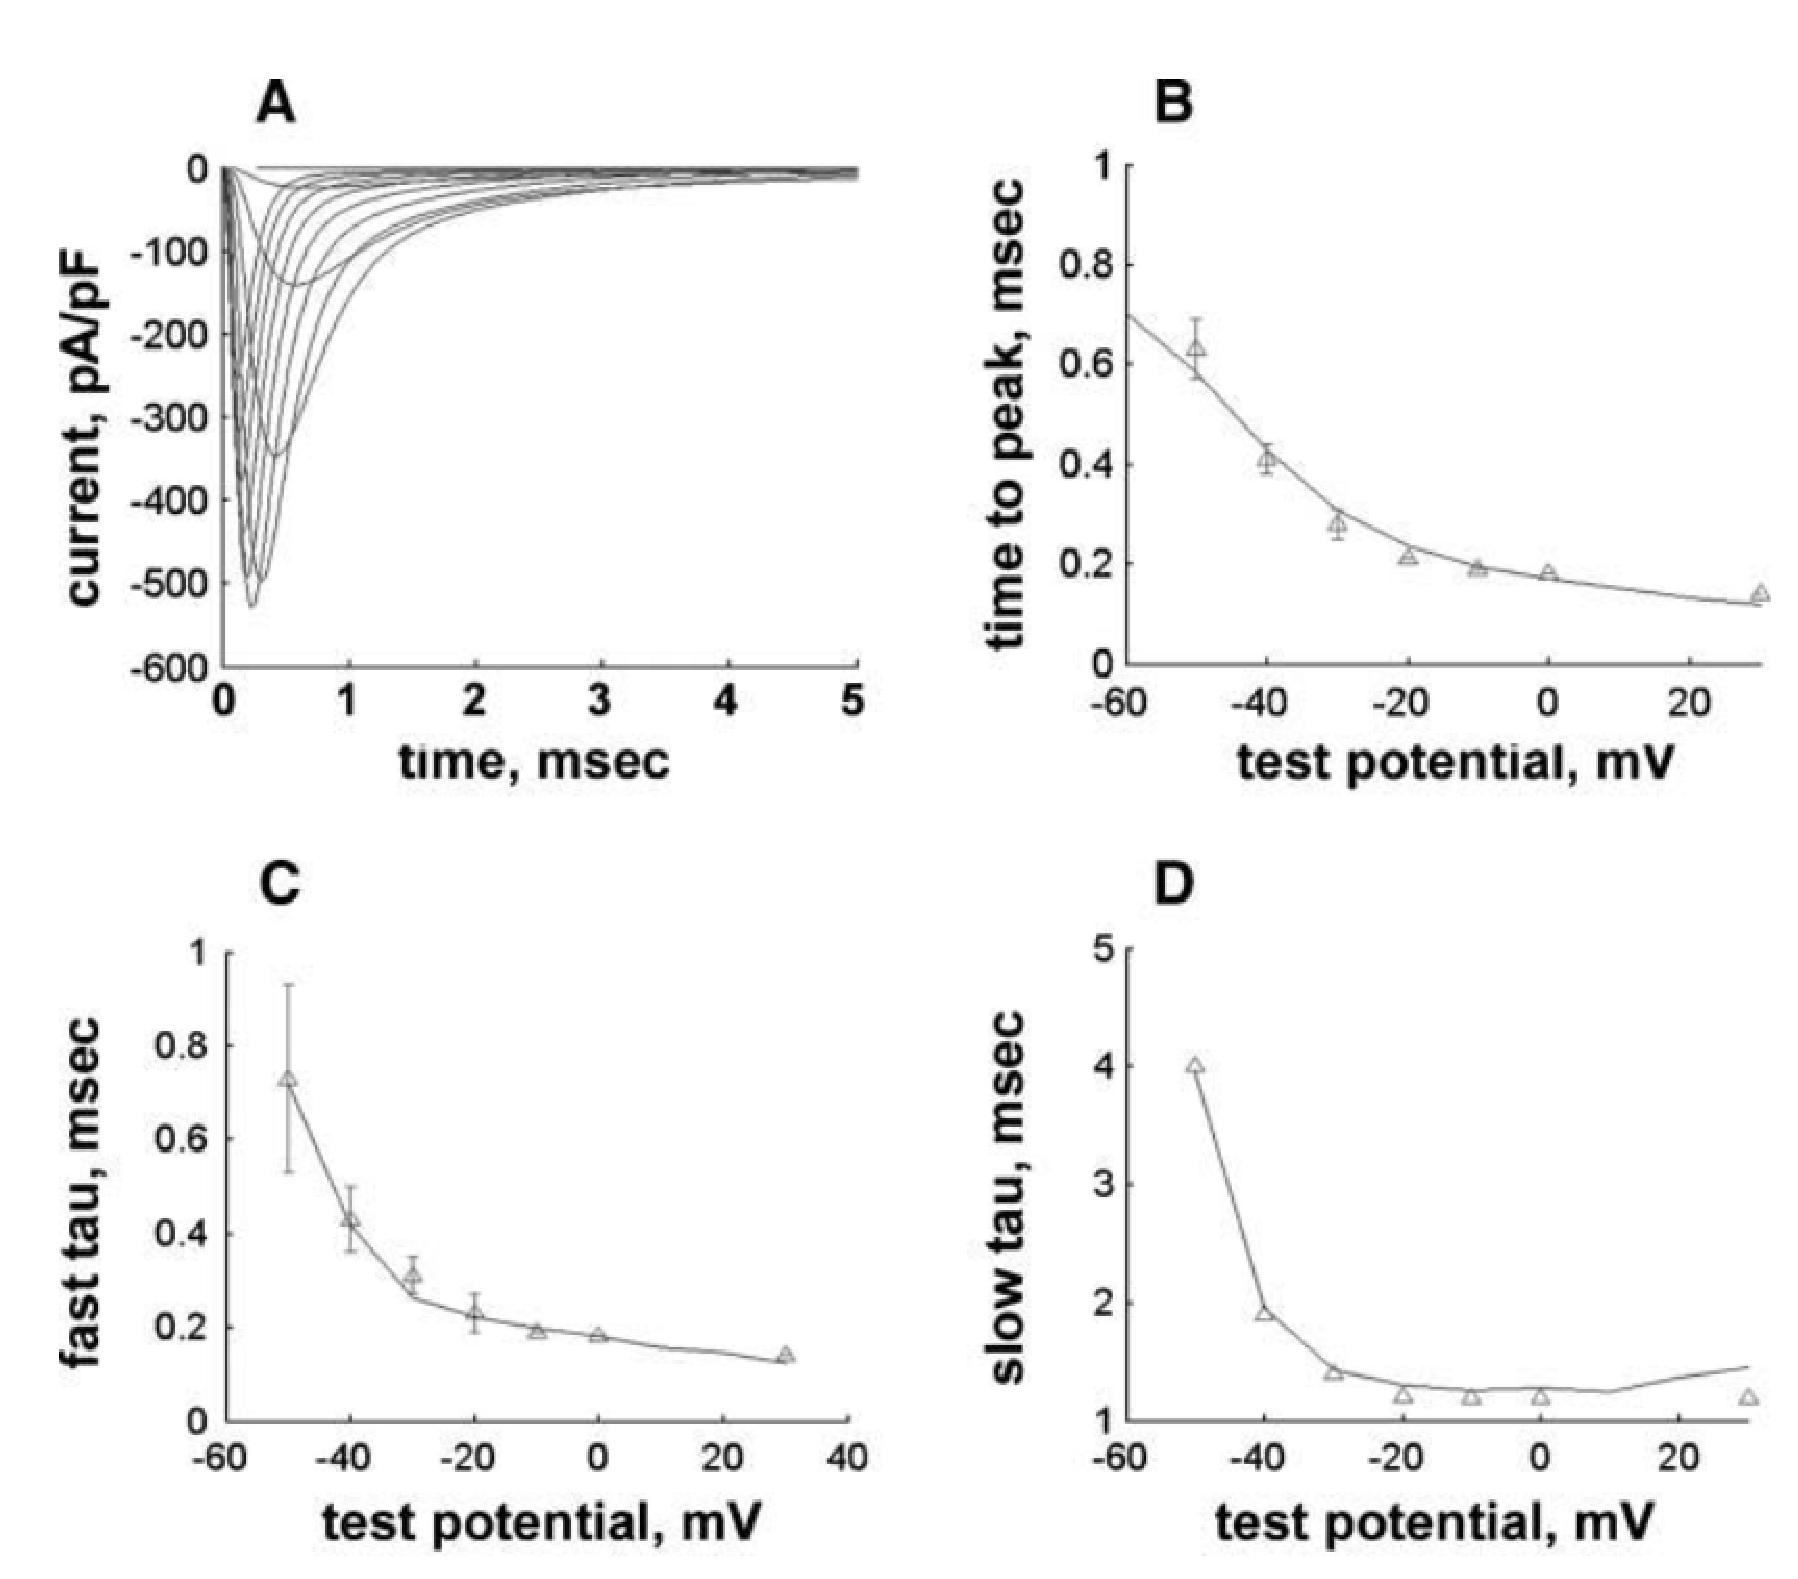
\includegraphics[height=5cm]{./images/Iyer2004_Ina.eps}}
  \caption{Simulated (solid line) vs. experimentally measured $I_\na$ currents
  from \citep{nagatomo1998, wang2000} (at 33$^\circ$C)}\label{fig:Iyer2004_Ina}
\end{figure}
 
The $I_\na$ density is also adjusted to reproduce the measurement of AP
amplitude which is 126mV at 1Hz pacing (in the midrange of experimental data
\citep{li1998, nabauer1996}), and phase 0 upstroke velocity $(dV_m/dt)_\max$
(Volt/sec) to be 350 (V/s), similar to values measured experimentally in human
ventricular subepicardium and midmyocardium \citep{drouin1995, pereon2000}.













